
\twocolumn[{%
\renewcommand\twocolumn[1][]{#1}%
\maketitle
\begin{center}
    \centering
    \vspace{-4mm}
    \counterwithin{figure}{section}
    % \renewcommand\thefigure{A\arabic{figure}}
    \captionsetup{type=figure}
    \begin{minipage}{0.27\linewidth}
    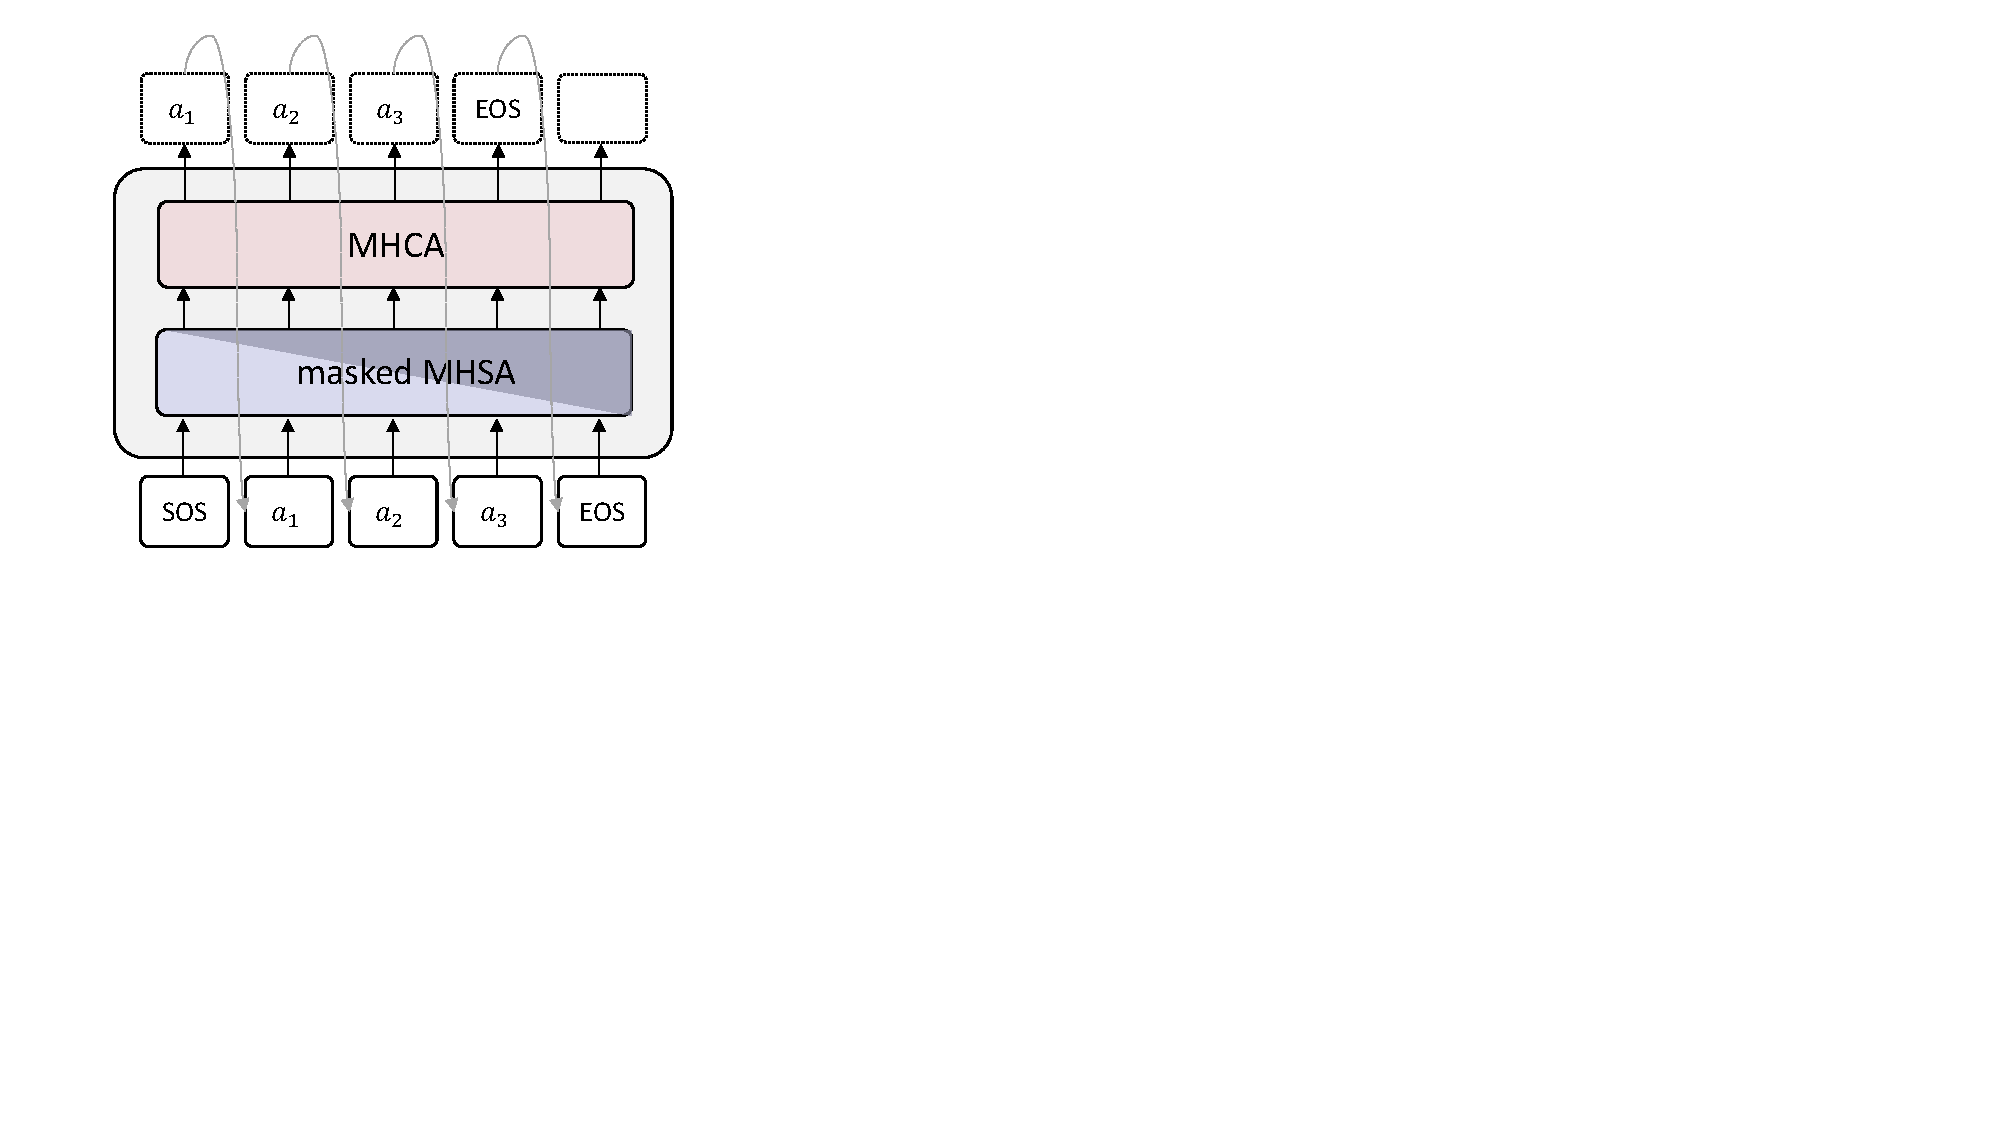
\includegraphics[width=\textwidth]{Figures/pdf/futr-a.pdf}
    \centering\small{(a) FUTR-A}
    \end{minipage}\hfill
    \begin{minipage}{0.27\linewidth}
    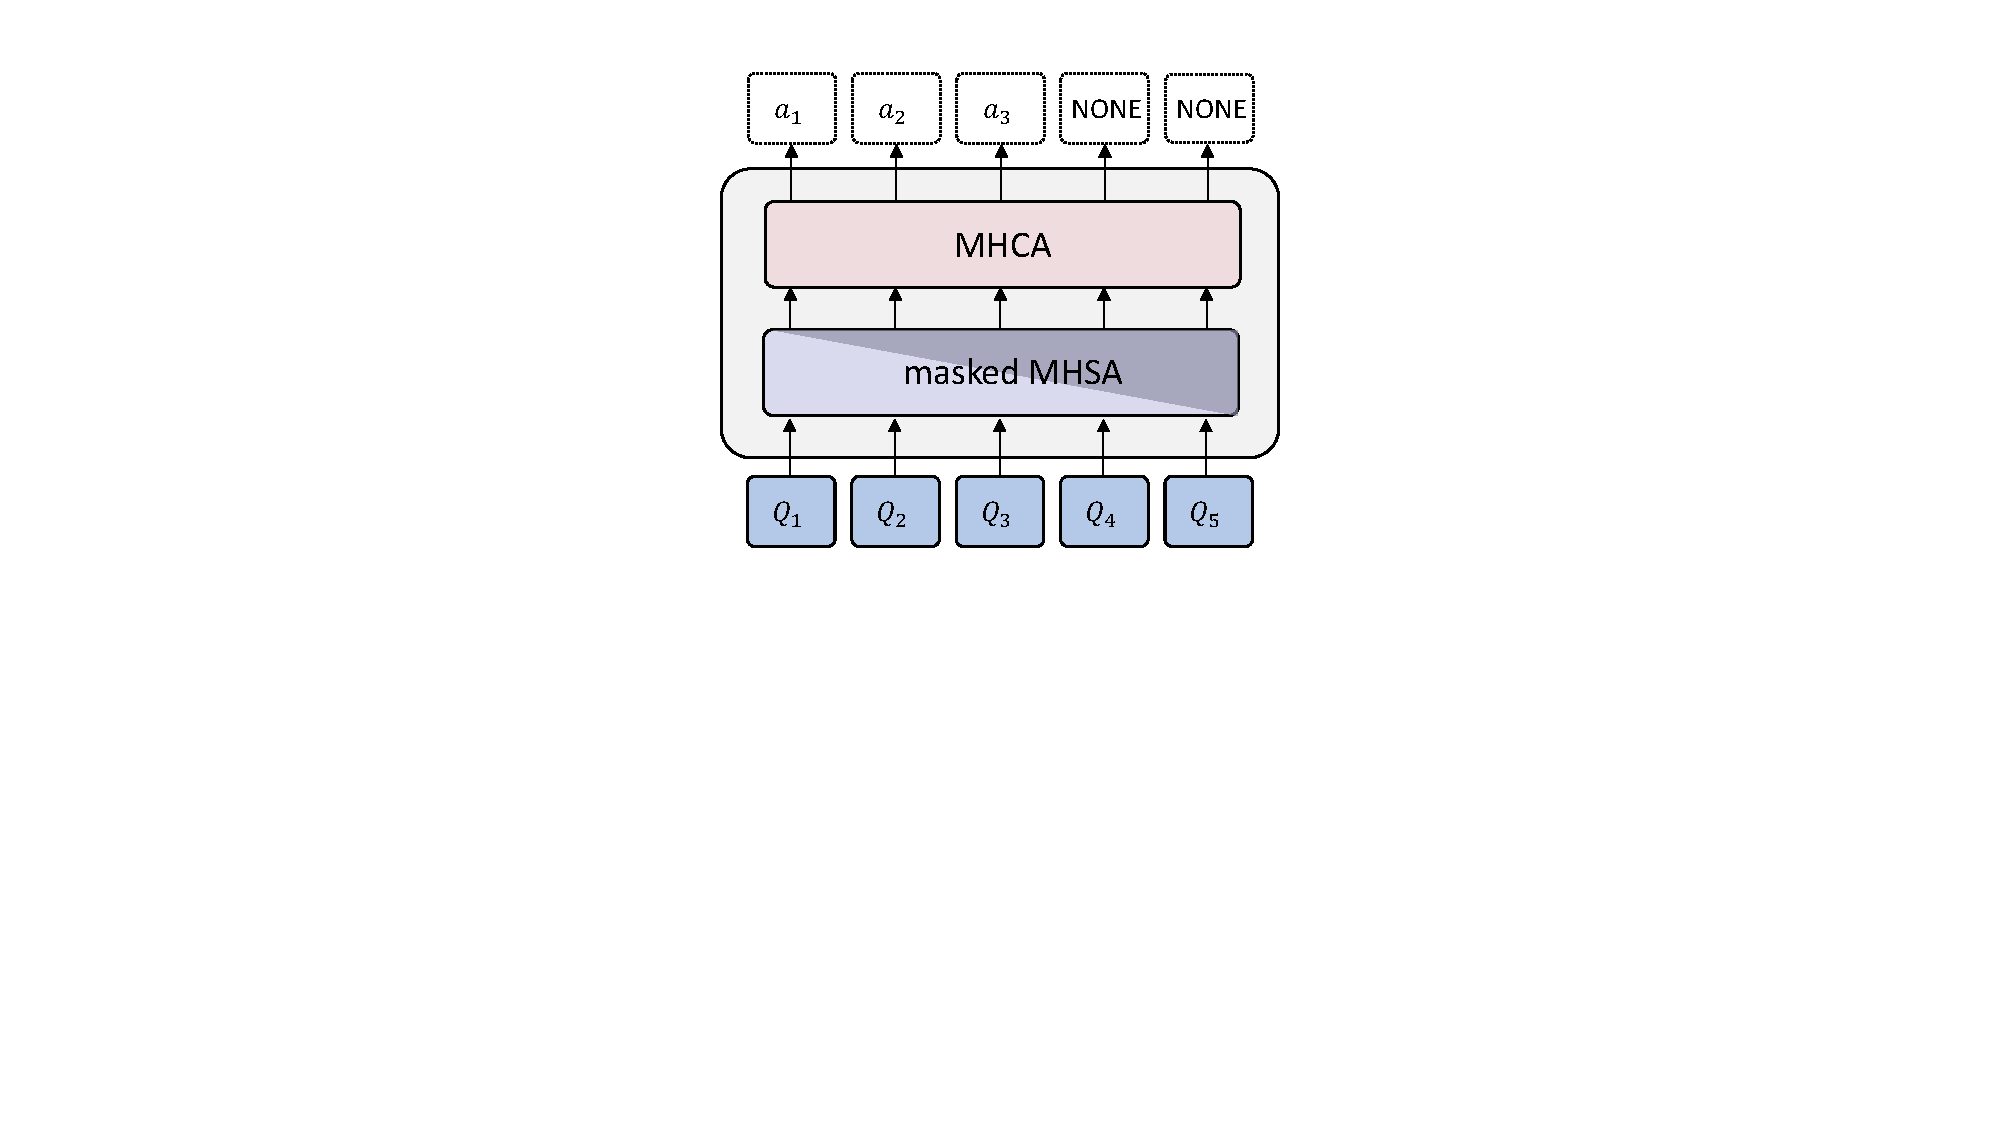
\includegraphics[width=\textwidth]{Figures/pdf/futr-m.pdf}
    \centering\small{(b) FUTR-M}
    \end{minipage}\hfill
    \begin{minipage}{0.27\linewidth}
    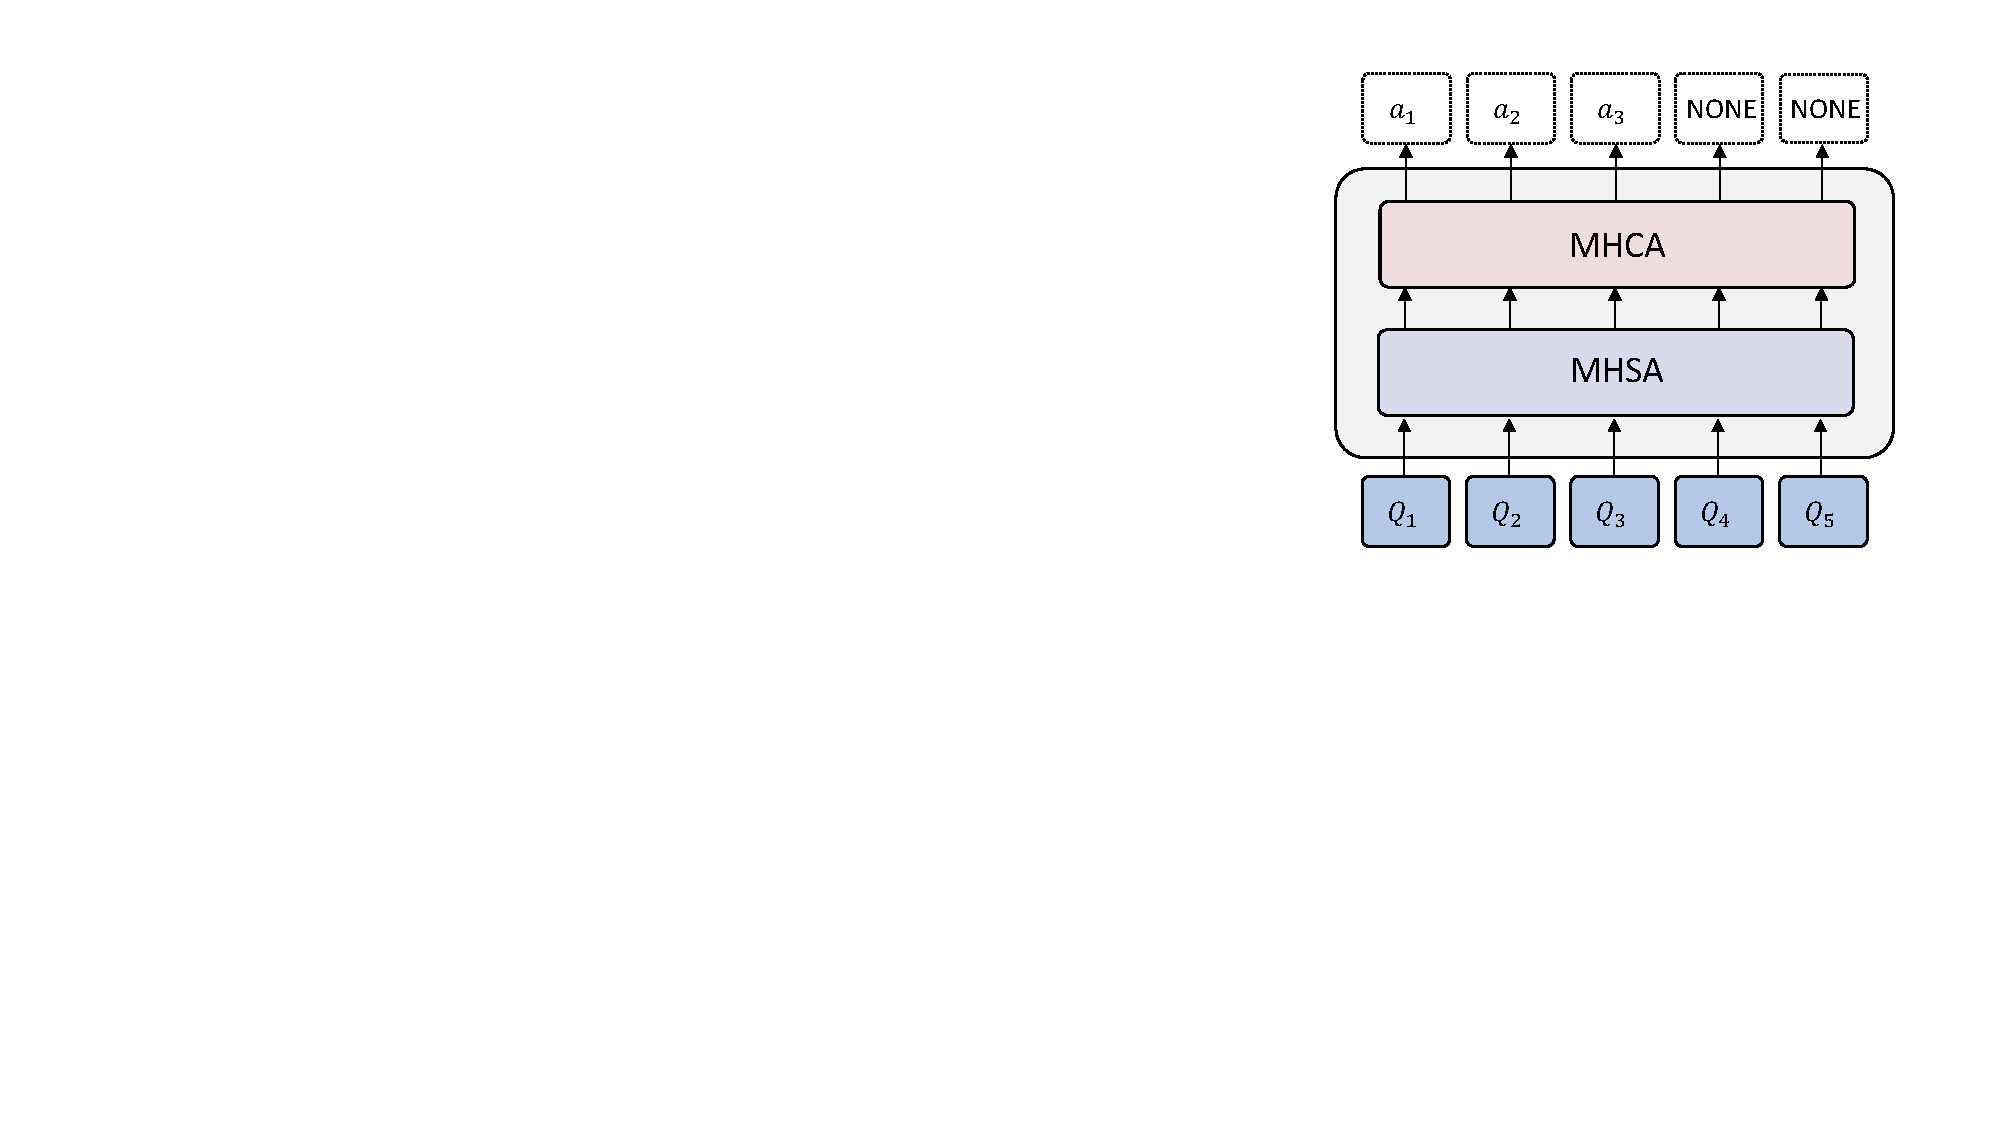
\includegraphics[width=\textwidth]{Figures/pdf/futr.pdf}
    \centering\small{(c) FUTR}
    \end{minipage}\hfill
    \begin{minipage}{0.15\linewidth}
    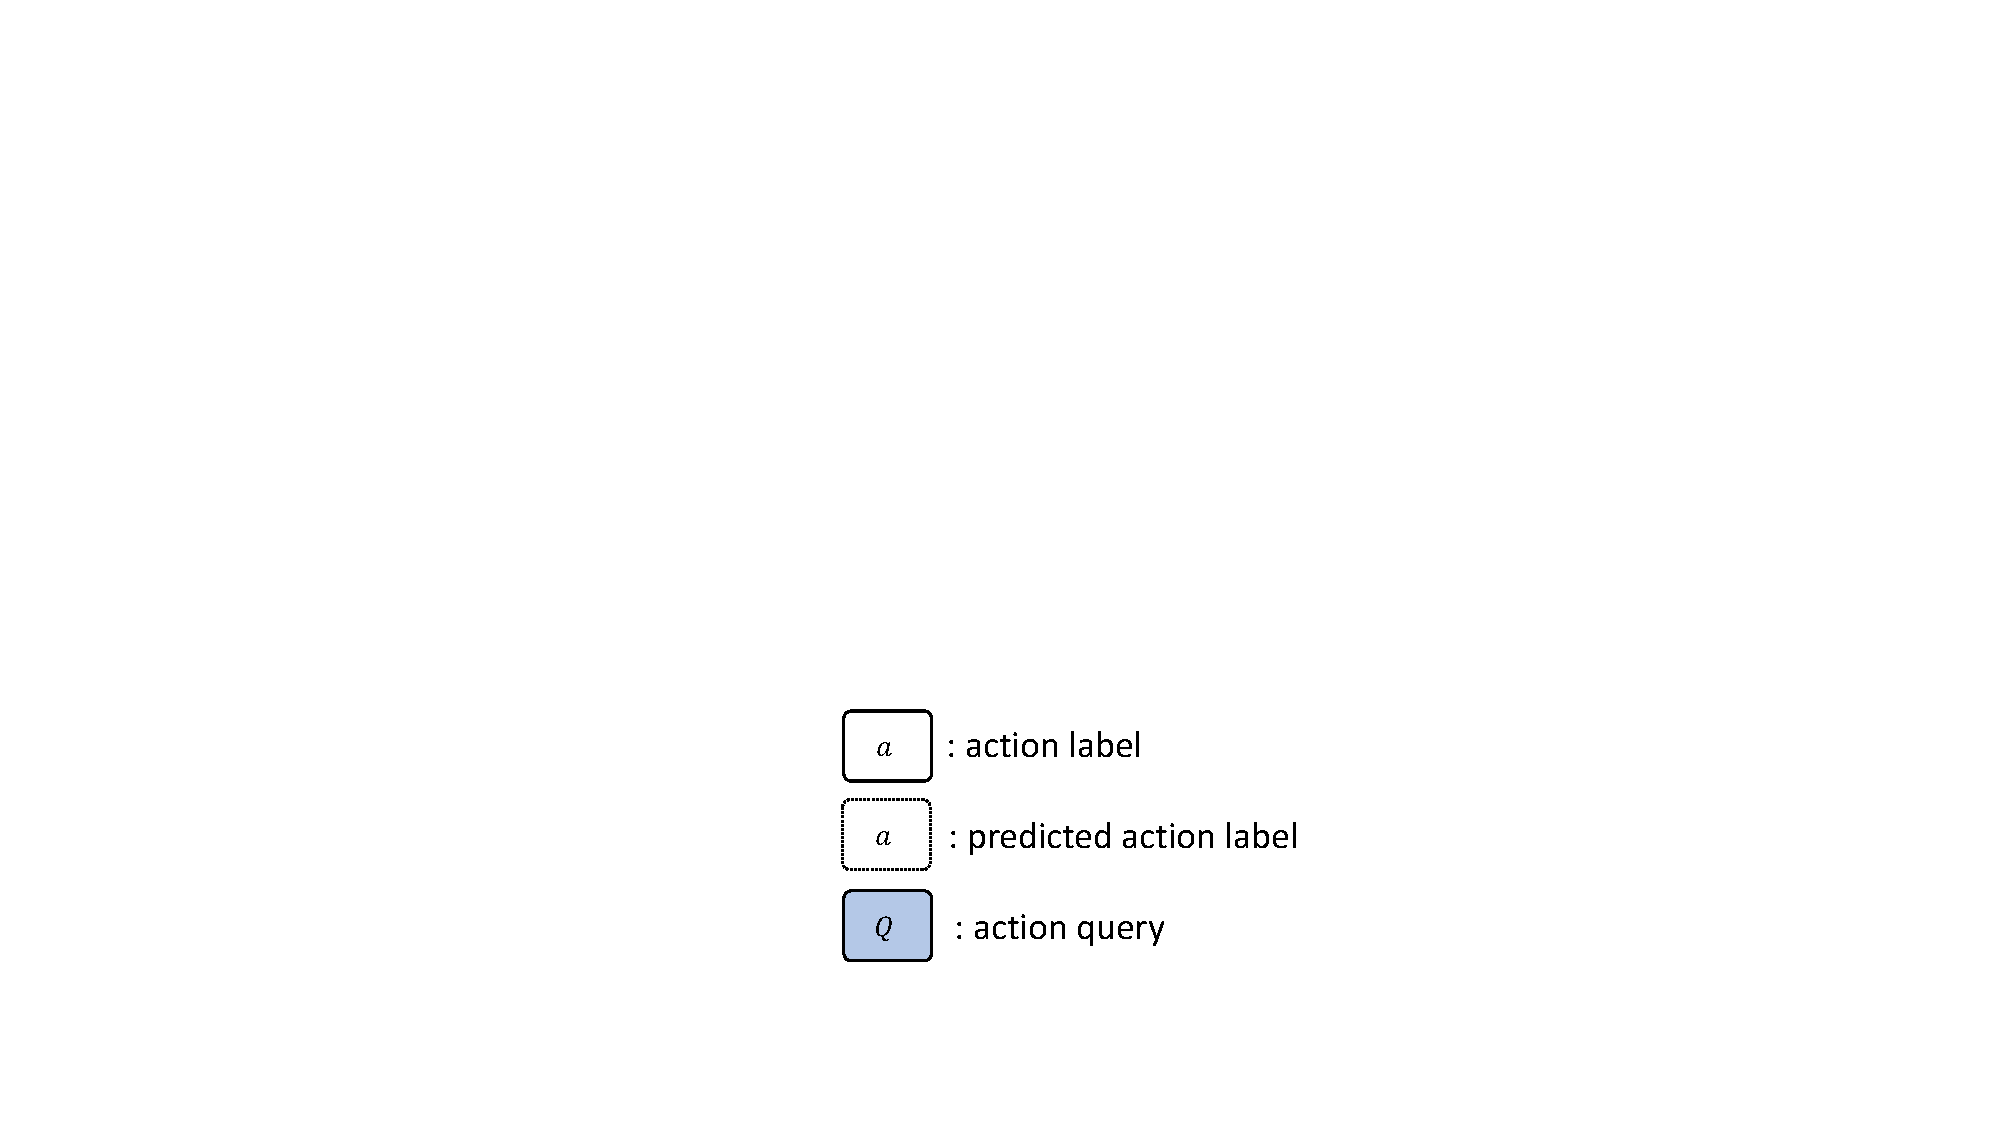
\includegraphics[width=\textwidth]{Figures/pdf/futr-idx.pdf}
    \end{minipage}\hfill
    \counterwithin{figure}{section}
    \renewcommand\thefigure{S\arabic{figure}}
    \caption{\textbf{\ours variants with different decoding strategies.}
    (a) \ours-A autoregressively anticipates future actions using the output action labels from the previous predictions as input and utilizes masked self-attention.
    (b) \ours-M is equivalent to \ours except for masked self-attention applied to action queries.
    (c) \ours remove a causal mask in MHSA, where query attends to past and future queries in the sequence. \ours-M and \ours anticipates action and duration for each query simultaneously.
    }
    % \vspace{-1mm}
    \label{fig:parallel}
\end{center}%
}]
